\section{Versuchsaufbau und Durchführung}
\label{sec:Durchführung}
Der gesamte Versuchsaufbau befindet sich in der Abbildung \ref{fig:optischeraufbau}. Das Licht von der Kondensorlinse wird durch einen Spalt geleitet, mit einer Linse gebündelt und dann an einem Prisma gebrochen. Die Abbildungslinse muss so justiert werden, so dass ein scharfes Bild entstehen kann. Mit Hilfe der Geradsichtprima wird das Licht in verschiedenen Spektrallinien aufgespaltet, sodass sie zu unterscheiden sind. 
Dazu gibt es auch noch eine Mattscheibe, die vor der Photokathode gestellt werden muss, um die verschiedenen Spektrallinien zu beobachten. 

Zuerst wird die Gegenfeldmethode untersucht, um die Energie des ausgelösten Elektronen zu bestimmen. Für diese Methode werden $5$ verschiedene Spektrallinien gebraucht. Es werden jeweils $10$ Messwerte für die Spannung $U$ und den Strom $I$ notiert, wobei mit abnehmender Spannung der Strom zunimmt.
Zu der anderen zweiten Messung wird eine Wellenlänge von ca. $\lambda = \SI{579,1}{\nano\meter}$ benötigt, um den Photostrom in Abhängigkeit der Spannung zwischen der Anode und Kathode zu messen. Dafür muss die Spannung zwischen $\SI{-20}{\volt}$ und $\SI{+20}{\volt}$ hochgeregelt werden. Zwischen den Bereich $\SI{1}{\volt}$ und $\SI{2}{\volt}$ werden die Messwerte in zweier Schritte notiert. Insgesamt werden aber mehr als 30 Messwerte notiert.
\begin{figure}[h!]
	\centering
	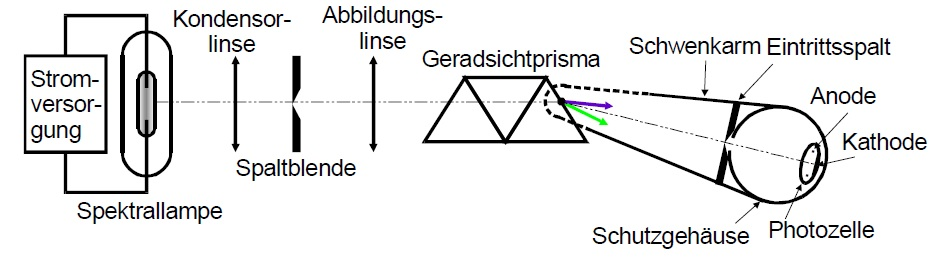
\includegraphics[width=0.9\linewidth]{../../OptischerAufbau}
	\caption{Genereller Versuchsaufbau zur Untersuchung des Photoeffektes, \cite[4]{anleitung500}.}
	\label{fig:optischeraufbau}
\end{figure}
